\setbeamertemplate{block begin}{
  \vskip.75ex
  \begin{beamercolorbox}[rounded=true,shadow=true,leftskip=1cm,colsep*=.75ex]{block title}%
    \usebeamerfont*{block title}\insertblocktitle
  \end{beamercolorbox}%
  {\ifbeamercolorempty[bg]{block body}{}{\nointerlineskip\vskip-0.5pt}}%
  \usebeamerfont{block body}%
  \begin{beamercolorbox}[rounded=true,shadow=true,colsep*=.75ex,sep=.75ex, vmode]{block body}%
    \ifbeamercolorempty[bg]{block body}{\vskip-.25ex}{\vskip-.75ex}\vbox{}%
    \begin{adjustwidth}{0.8cm}{0.4cm}
  }
  \setbeamertemplate{block end}{
  \end{adjustwidth}
  \end{beamercolorbox}
}


\begin{block}{\large \smash{1. Introduction}\vphantom{Introduction}}

\begin{columns}[T]
\begin{column}{0.01\linewidth}\end{column}
\begin{column}{.48\linewidth}
\alert{Dependability} of computer systems is becoming more and more important.

\ 

\begin{figure}[h!]
\hfill
\subfigure[Windows blue screen]{
\newcommand{\bluescreen}[1]{\color{white}\texttt{#1}}

\tikzstyle{background rectangle}= [fill=blue!60!black, draw=white]
\begin{tikzpicture}[scale=1, show background rectangle]
\node[] (s_1) {\scalebox{0.25}{
\begin{minipage}{42cm}
\noindent\\\noindent\\\noindent\\\noindent\\\noindent\\\noindent\\
\noindent{\color{blue!60!black}x}\texttt{\ \ \ \ \ \ \ \ \ \ \ \ \ \ \ \ \ \ \ \ \ \ \ \ \ \ \ \ \ \ }\colorbox{gray}{\color{blue!60!black}\texttt{\phantom{.}Windows\phantom{.}}\vphantom{$\sum_{n=0}^\infty$}}\\\noindent\\
\bluescreen{A fatal exception 0E has occurred at 0137:BFFA21C9. The current}\\
\bluescreen{application will be terminated.}\\
\noindent\\
\bluescreen{* Press any key to terminate the current application.}\\
\bluescreen{* Press CTRL+ALT+DEL again to restart your computer. You will}\\
\bluescreen{\ \ lose any unsaved information in all application.}\\
\noindent\\
\bluescreen{\ \ \ \ \ \ \ \ \ \ \ \ \ \ \ \ \ \ \ \ \ Press any key to continue}
\noindent\\\noindent\\\noindent\\\noindent\\\noindent\\\noindent\\
\end{minipage}
}};
\end{tikzpicture}
}
\hfill
\subfigure[Ariane 5 crash]{
\raisebox{0.08cm}{
%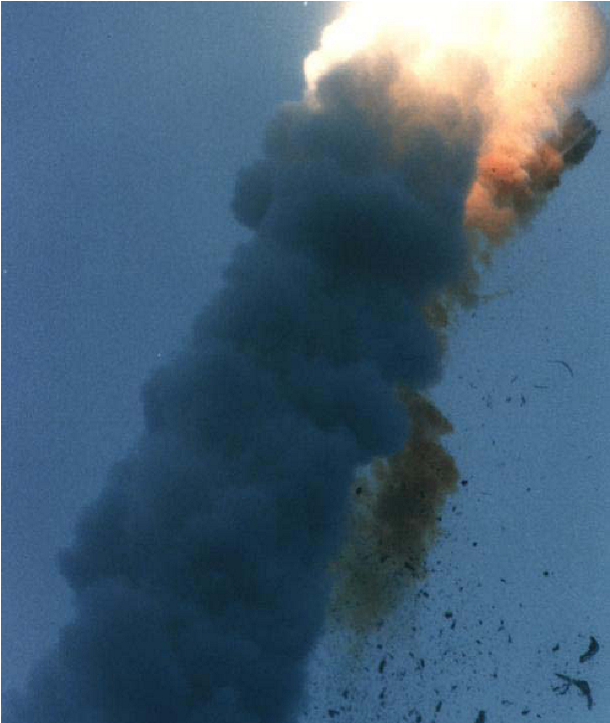
\includegraphics[scale=0.573]{figures/ariane5-2.png}
}}
\hfill
{}
\end{figure}
%%% Eind plaatjes

\noindent \\[65pt]

Our aim is to use \alert{formal methods} to improve system quality.

\end{column}
\begin{column}{.02\linewidth}
\begin{tabular}{cc|}
&\\
&\\
&\\
&\\
&\\
&\\
&\\
&\\
&\\
&\\
&\\
\end{tabular}
\end{column}
\begin{column}{.48\linewidth}
A popular solution is \alert{model checking}; verifying \alert{properties} of a system by constructing a \alert{model} and ranging over its \alert{state space}. \

\vskip-20pt

\begin{columns}
\begin{column}{0.02\linewidth}\end{column}
\begin{column}{.48\linewidth}
\begin{figure}[h!]
\subfigure[An overview of model checking]{
\begin{tikzpicture}[scale=0.7, transform shape] 
\node[] (sinit) {};
\node[cloud, fill=white, draw=black, cloud puffs=15, aspect=2.5, inner sep=0pt, cloud puff arc=120, text=black] (s0) [right of=sinit, node distance=7cm] {\bf $\mathrlap{\text{\ \ \ \ System}}$\phantom{Requirements}}; 
\node[smallrectangle] (s1) [below of=s0, node distance=7cm] {$\mathrlap{\text{\ \:Model}}\phantom{Property}$};
\node[cloud, fill=white, draw=black, cloud puffs=15, aspect=2.5, inner sep=0pt, cloud puff arc=120, text=black] (s2) [right of=s0, node distance=15cm] {\bf Requirements}; 
\node[smallrectangle] (s3) [below of=s2, node distance=7cm] {Property};
\draw[->] (s0) edge (s1);
\draw[->] (s2) edge (s3);
\node[] (temp) [below of=s1, node distance=6cm] {};
\node[smallrectangle] (s4) [right of=temp, node distance=7.5cm] {Model checker};
\draw[->] (s1) edge (s4);
\draw[->] (s3) edge (s4);
\node[oval, inner sep=0.4cm, fill=red] (s5) [left of=s4, node distance=9cm] {Fail};
\node[oval, inner sep=0.4cm, fill=green] (s6) [right of=s4, node distance=9cm] {Pass};
\draw[->] (s4) edge (s5);
\draw[->] (s4) edge (s6);
\draw[->] (s5) edge (s1);

\end{tikzpicture}
}
\end{figure}
\end{column}
\begin{column}{.12\linewidth}\end{column}
\begin{column}{.36\linewidth}
\begin{figure}
\vskip23pt
\subfigure{
\begin{tikzpicture}[scale=1.25, transform shape, show background rectangle, node distance=2.5cm, descr/.style={fill=white,inner sep=2.5pt}]
 
	   \path (0.5,0) node[smallstate, fill=green] (s_0) {}
             (1.5,-1) node [smallstate, fill=green] (s_1) {}
	   (2.1, 0.5) node [smallstate, fill=green] (s_2) {}
	   (2.8, -0.25) node [smallstate, fill=green] (s_3) {}
	   (4, 0.45) node [smallstate, fill=green] (s_4) {}
	   (3.3, -1) node [smallstate, fill=green] (s_5) {}
	   (4.2, -0.8) node [smallstate, fill=green] (s_6) {}
	   (1.1, -2.4) node [smallstate, fill=green] (s_7) {}
	   (2.5, -2.0) node [smallstate, fill=green] (s_8) {}
	   (3.55, -1.75) node [smallstate, fill=green] (s_9) {}
	   (4.5, -2.3) node [smallstate, fill=green] (s_10) {}
	  (2.4, -3) node [smallstate, fill=green] (s_11) {}
	  (3.8, -3.2) node [smallstate, fill=green] (s_12) {};
	   
	   	
	\draw[->, ultra ultra thick ] (s_0) edge (s_1);
	\draw[->, ultra ultra thick] (s_1) edge (s_2);
	\draw[->, ultra ultra thick] (s_1) edge (s_3);
	\draw[->, ultra ultra thick] (s_3) edge (s_4);
	\draw[->, ultra ultra thick] (s_4) edge (s_5);
	\draw[->, ultra ultra thick] (s_4) edge (s_6);
	\draw[->, ultra ultra thick] (s_1) edge (s_7);
	\draw[->, ultra ultra thick] (s_7) edge (s_8);
	\draw[->, ultra ultra thick] (s_8) edge (s_9);
	\draw[->, ultra ultra thick] (s_8) edge (s_11);
	\draw[->, ultra ultra thick] (s_9) edge (s_10);
	\draw[->, ultra ultra thick] (s_10) edge (s_12);
	
\end{tikzpicture}
}
%
\subfigure[\qquad \qquad \qquad \qquad \ $\mathllap{\text{The output of model checking}}$]{
\begin{tikzpicture}[scale=1.25, transform shape, show background rectangle, node distance=2.5cm, descr/.style={fill=white,inner sep=2.5pt}]
      \path
    	(0.5,0) node[smallstate, fill=green] (s_0) {}
             (1.5,-1) node [smallstate, fill=green] (s_1) {}
	   (2.1, 0.5) node [smallstate, fill=green] (s_2) {}
	   (2.8, -0.25) node [smallstate, fill=green] (s_3) {}
	   (4, 0.45) node [smallstate, fill=green] (s_4) {}
	   (3.3, -1) node [smallstate, fill=green] (s_5) {}
	   (4.2, -0.8) node [smallstate, fill=green] (s_6) {}
	   (1.1, -2.4) node [smallstate, fill=green] (s_7) {}
	   (2.5, -2.0) node [smallstate, fill=green] (s_8) {}
	   (3.55, -1.75) node [smallstate, fill=green] (s_9) {}
	   (4.5, -2.3) node [smallstate, fill=green] (s_10) {}
	  (2.4, -3) node [smallstate, fill=red] (s_11) {}
	  (3.8, -3.2) node [smallstate, fill=green] (s_12) {};
	   	
	\draw[->, ultra ultra thick, color=blue, densely dotted] (s_0) edge (s_1);
	\draw[->, ultra ultra thick] (s_1) edge (s_2);
	\draw[->,ultra ultra thick] (s_1) edge (s_3);
	\draw[->,ultra ultra thick] (s_3) edge (s_4);
	\draw[->,ultra ultra thick] (s_4) edge (s_5);
	\draw[->,ultra ultra thick] (s_4) edge (s_6);
	\draw[->, ultra ultra thick, color=blue, densely dotted] (s_1) edge (s_7);
	\draw[->, ultra ultra thick, color=blue, densely dotted] (s_7) edge (s_8);
	\draw[->,ultra ultra thick] (s_8) edge (s_9);
	\draw[->, ultra ultra thick, color=blue, densely dotted] (s_8) edge (s_11);
	\draw[->,ultra ultra thick] (s_9) edge (s_10);
	\draw[->,ultra ultra thick] (s_10) edge (s_12);
		
\end{tikzpicture}
}
\end{figure}

\begin{textblock}{5}(80.5,36.3)
\parbox{5cm}{\raggedleft Pass:}
\end{textblock}
\begin{textblock}{5}(80.5,47.1)
\parbox{5cm}{\raggedleft Fail:}
\end{textblock}


\end{column}
\begin{column}{0.02\linewidth}\end{column}
\end{columns}
\end{column}
\begin{column}{.01\linewidth}\end{column}
\end{columns}
\end{block}	
